\newpage\subsection*{1551 Worksheet 6 Answers}

\SolutionsStatement

\begin{enumerate}
    
    \item \begin{enumerate}
    
    	\item A solution is shown below. Many acceptable answers.
        
        \begin{center}
    	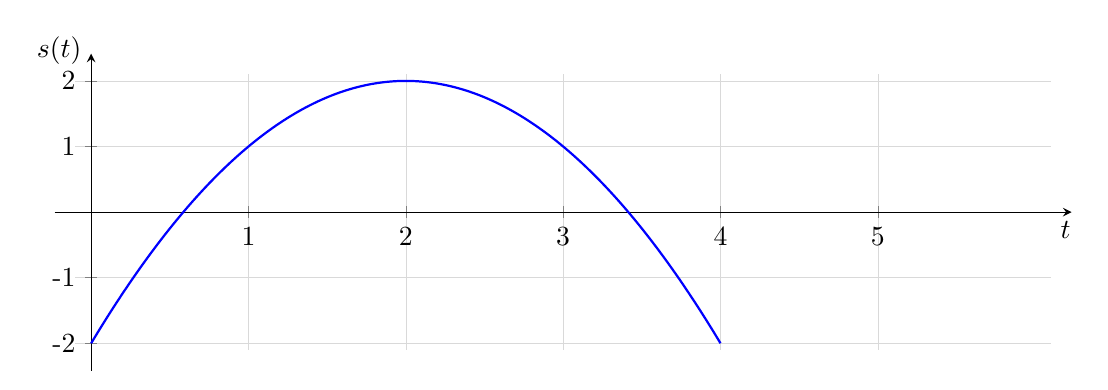
\begin{tikzpicture}[domain=0:6] 
        \begin{axis}[
        width=5.5in,
        height=2in,
        grid=both,
        grid style={line width=.2pt, draw=gray!30},
        clip=false,
        axis lines=middle,
        xmin=-0.1,xmax=6.1,
        ymin=-2.1,ymax=2.1,
        xtick={0,1,2,3,4,5},
        xticklabels={0,1,2,3,4,5},
        ytick={-2,-1,0,1,2},
        yticklabels={-2,-1,0,1,2},
        axis line style={shorten >=-7.5pt, shorten <=-7.5pt},
        xlabel=$t$,
        ylabel=$s(t)$,
        xlabel style={at={(ticklabel* cs:1)},anchor=north west},
        ylabel style={at={(ticklabel* cs:1)},anchor=south east}
        ]
        \addplot[samples=100,domain=0:4,smooth, thick, blue] {2 - (x-2)*(x-2)} node[pos=1] (endofplotsquare) {}; 
        \end{axis}
    \end{tikzpicture}   
    \end{center}    
        
        \item Many acceptable answers, including $s(t) = 2 - (t - 2)^2$. 
    
	\end{enumerate}
    
    \item \begin{enumerate}
    
    	\item The velocity and speed are shown below. 
        \begin{center}
    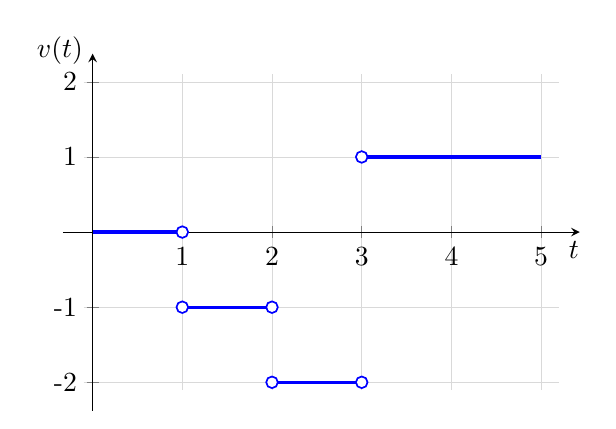
\begin{tikzpicture}[domain=0:5.2] 
        \begin{axis}[
        width=3in,
        height=2.2in,
        grid=both,
        grid style={line width=.2pt, draw=gray!30},
        clip=false,
        axis lines=middle,
        xmin=-0.1,xmax=5.2,
        ymin=-2.1,ymax=2.1,
        xtick={0,1,2,3,4,5},
        xticklabels={0,1,2,3,4,5},
        ytick={-2,-1,0,1,2},
        yticklabels={-2,-1,0,1,2},
        axis line style={shorten >=-7.5pt, shorten <=-7.5pt},
        xlabel=$t$,
        ylabel=$v(t)$,
        xlabel style={at={(ticklabel* cs:1)},anchor=north west},
        ylabel style={at={(ticklabel* cs:1)},anchor=south east}
        ]
        \addplot[samples=100,domain=0:1,smooth, very thick, blue] {0} node[pos=1] (endofplotsquare) {};
        \addplot[samples=100,domain=1:2,smooth, very thick, blue] {-1} node[pos=1] (endofplotsquare) {};
        \addplot[samples=100,domain=2:3,smooth, very thick, blue] {-2} node[pos=1] (endofplotsquare) {};        
        \addplot[samples=100,domain=3:5,smooth, very thick, blue] {1} node[pos=1] (endofplotsquare) {};        
        \addplot[blue,mark=o,thick] coordinates {(1,+0)};
        \addplot[blue,mark=o,thick] coordinates {(1,-1)};
        \addplot[blue,mark=o,thick] coordinates {(2,-1)};
        \addplot[blue,mark=o,thick] coordinates {(2,-2)};
        \addplot[blue,mark=o,thick] coordinates {(3,-2)};
        \addplot[blue,mark=o,thick] coordinates {(3,+1)};        
        \addplot[white,mark=*, mark size=1.5] coordinates {(1,+0)};
        \addplot[white,mark=*, mark size=1.5] coordinates {(1,-1)};
        \addplot[white,mark=*, mark size=1.5] coordinates {(2,-1)};
        \addplot[white,mark=*, mark size=1.5] coordinates {(2,-2)};
        \addplot[white,mark=*, mark size=1.5] coordinates {(3,-2)};
        \addplot[white,mark=*, mark size=1.5] coordinates {(3,+1)};
        \end{axis}
    \end{tikzpicture}   
    \end{center}    
    \vspace{12pt}
    \begin{center}
    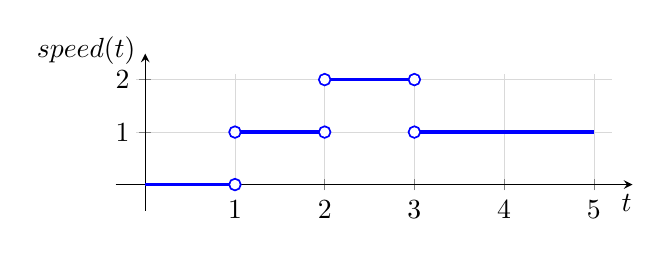
\begin{tikzpicture}[domain=0:5.2] 
        \begin{axis}[
        width=3in,
        height=1.2in,
        grid=both,
        grid style={line width=.2pt, draw=gray!30},
        clip=false,
        axis lines=middle,
        xmin=-0.1,xmax=5.2,
        ymin=-0.1,ymax=2.1,
        xtick={0,1,2,3,4,5},
        xticklabels={0,1,2,3,4,5},
        ytick={-2,-1,0,1,2},
        yticklabels={-2,-1,0,1,2},
        axis line style={shorten >=-7.5pt, shorten <=-7.5pt},
        xlabel=$t$,
        ylabel=$speed(t)$,
        xlabel style={at={(ticklabel* cs:1)},anchor=north west},
        ylabel style={at={(ticklabel* cs:1)},anchor=south east}
        ]
        \addplot[samples=100,domain=0:1,smooth, very thick, blue] {0} node[pos=1] (endofplotsquare) {};
        \addplot[samples=100,domain=1:2,smooth, very thick, blue] {1} node[pos=1] (endofplotsquare) {};
        \addplot[samples=100,domain=2:3,smooth, very thick, blue] {2} node[pos=1] (endofplotsquare) {};        
        \addplot[samples=100,domain=3:5,smooth, very thick, blue] {1} node[pos=1] (endofplotsquare) {};        
        \addplot[blue,mark=o,thick] coordinates {(1,0)};
        \addplot[blue,mark=o,thick] coordinates {(1,1)};
        \addplot[blue,mark=o,thick] coordinates {(2,1)};
        \addplot[blue,mark=o,thick] coordinates {(2,2)};
        \addplot[blue,mark=o,thick] coordinates {(3,2)};
        \addplot[blue,mark=o,thick] coordinates {(3,1)};        
        \addplot[white,mark=*, mark size=1.5] coordinates {(1,0)};
        \addplot[white,mark=*, mark size=1.5] coordinates {(1,1)};
        \addplot[white,mark=*, mark size=1.5] coordinates {(2,1)};
        \addplot[white,mark=*, mark size=1.5] coordinates {(2,2)};
        \addplot[white,mark=*, mark size=1.5] coordinates {(3,2)};
        \addplot[white,mark=*, mark size=1.5] coordinates {(3,1)};
        \end{axis}
    \end{tikzpicture}   
    \end{center}    
        
        \item Speed is constant over $[0,1)\cup(1,2)\cup(2,3)\cup(3,5]$. At $t=0$ and $t = 5$, we are using the concept of differentiability on an interval, from Section 3.2. For more details see textbook, page 130. Or see lecture slides for section 3.2, slide 5. Or see lecture slides for section 3.4, slide 10. 
        
        \item Velocity is undefined at times $t = 1,2,3$. 
        
        \item Acceleration, wherever it is defined, is always zero because the velocity is piecewise constant. 
    
	\end{enumerate}
    
    \item \begin{enumerate}
    
    	\item False. Counterexample: $f = x + 10$, $g = 2x$ over $x\in(0,1)$.
    
        \item False. Counterexample: $f = x^2$.
        
        \item False. Counterexample: $f = \sin(t)$. Another counterexample is $f=2 - (t-1)^2$, which is the same function in question 1b.
    
	\end{enumerate}
    
    \item \begin{align*}
    	y'(x) &= \ddx \frac{2e^x}{x^2-1} \\
        &= \ddx 2e^x(x^2-1)^{-1} \\
        &= 2e^x (x^2 -1)^{-1} - 2e^x (x^2 - 1)^{-2}(2x) \\
        y'(0) &= 2e^0 (0^2 -1)^{-1} - 2e^0 (0^2 - 1)^{-2}(2\cdot 0) = -2 \\
        y(0) &= \frac{2e^x}{x^2-1} = -2 \\
        y - y(0) &= y'(0)(x-x_0) \\
        y - (-2) &= -2(x-0) \\    
        y &= -2x -2
    \end{align*}
    
    
    \begin{enumerate}
    	\item $y = 1 + f(x^2) g(h(x))$: 
        \begin{align*}
        	y' 
            &= 0 + \ddx  f(x^2) g(h(x)) \\
            &= 2xf'(x^2) g(h) + f(x^2)g'(h)h'
        \end{align*}
        \item $y = \frac{3+9\tan x}{\sec x}$:
        \begin{align*}
        	y' 
            &= \ddx \frac{3+9\tan x}{\sec x} \\
            &= \ddx \left(\frac{3}{\sec x} + \frac{9\tan x}{\sec x} \right)\\
            &= \ddx \left( 3\cos x + 9\sin x \right)\\
            &= -3\sin x + 9\cos x 
        \end{align*}        
    \end{enumerate}    
\end{enumerate}